\documentclass[12pt, a4paper, oneside]{article}
\usepackage{amsmath,amsthm,amssymb,graphicx}
\usepackage{float}
% \usepackage{algorithm}
% \usepackage{algorithmic}
\usepackage{pythonhighlight}

\title{\textbf{CS2601} Linear and Convex Optimization Project Report \\-- Implementing the Water-filling Algorithm}
\date{\today}

\author{Xuankun Yang 523030910248}

\begin{document}

\maketitle
\tableofcontents

\section{Introduction}
In this project, we concentrate on \textit{The Water-filling Problem}. I implemented 3 different methods in my experiments.\\
In this report, we have 3 parts: \textit{Obectives of the Experiment}, \textit{Experimental Process} and \textit{Results and Analysis}.

\section{Obectives of the Experiment}
The convex optimization problem:
\begin{displaymath}
    \mbox{minimize } -\sum_{i=1}^{n}\log{(\alpha_i + x_i)}
\end{displaymath}
\begin{displaymath}
    \mbox{subject to } x \succeq 0 , \mathbf{1}^Tx = 1 , \alpha_i > 0
\end{displaymath}
Introducing Lagrange multipliers $\lambda^{\star} \in \mathbf{R}^n$ for the inequality constraints $x^{\star} \succeq 0$, 
and a multiplier $\nu^{\star} \in \mathbf{R}$ for the equality constraint $\mathbf{1}^Tx = 1$, 
we obtain the \textit{KKT} conditions:
\begin{displaymath}
    x^{\star} \succeq 0 ,  \mathbf{1}^Tx^{\star} = 1 , \lambda^{\star} \succeq 0 , \lambda_i^{\star}x_i^{\star} = 0 , i = 1, \dots ,n ,
\end{displaymath}
\begin{displaymath}
    -\frac{1}{\alpha_i + x_i^{\star}} - \lambda_i^{\star} + \nu^{\star} = 0,  i = 1, \dots ,n.
\end{displaymath}
We can directly solve these equations to find $x^{\star}, \lambda^{\star}$ and $\nu^{\star}$.\\
Noting that $\lambda^{\star}$ acts as a slack variable in the last equation, so it can be eliminated, leaving
\begin{displaymath}
    x^{\star} \succeq 0 ,  \mathbf{1}^Tx^{\star} = 1 , (\nu^{\star} - \frac{1}{\alpha_i + x_i^{\star}})x_i^{\star} = 0 , i = 1, \dots , n,
\end{displaymath}
\begin{displaymath}
    \nu^{\star} \geqslant \frac{1}{\alpha_i + x_i^{\star}} , i = 1, \dots ,n.
\end{displaymath}
Next, we make a discussion on $\nu^{\star}$
\begin{enumerate}
    \item 
    {
        If $\nu^{\star} < \frac{1}{\alpha_i}$, the last condition can hold only if $x_i^{\star} > 0$, 
        according to the third condition, $\nu^{\star} = \frac{1}{\alpha_i + x_i^{\star}}$\\
        Solving for $x_i^{\star}$, we conclude that $x_i^{\star} = \frac{1}{\nu^{\star}} - \alpha_i$, if $\nu^{\star} < \frac{1}{\alpha_i}$
    }
    \item 
    {
        If $\nu^{\star} \geqslant \frac{1}{\alpha_i}$, according to the third condition, $x_i^{\star} = 0$ must hold\\
        Therefore, $x_i^{\star} = 0$, if $\nu^{\star} \geqslant \frac{1}{\alpha_i}$
    }
\end{enumerate}
Thus, we have
\begin{displaymath}
    x_i^{\star} = \left\{ 
    \begin{array}{lcr}
            \frac{1}{\nu^{\star}} - \alpha_i ,  &  \nu^{\star} < \frac{1}{\alpha_i}\\
            0 , & \nu^{\star} \geqslant \frac{1}{\alpha_i}
    \end{array}
    \right.
\end{displaymath}
or, put more simply, $x_i^{\star} = \mbox{max}\{0, \frac{1}{\nu^{\star}} - \alpha_i\}$.\\
Substituting this expression for $x_i^{\star}$ into the condition $\mathbf{1}^Tx^{\star} = 1$, we obtain
\begin{displaymath}
    \sum_{i = 1}^{n}\mbox{max}\{0, \frac{1}{\nu^{\star}} - \alpha_i\} = 1
\end{displaymath}
\begin{figure}[H]
    \centering
    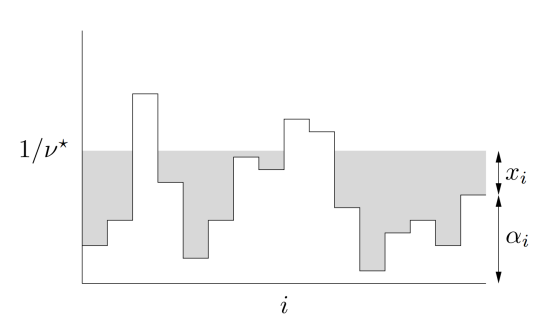
\includegraphics[width = 12cm]{illustration.png}
    \caption{Visualization}
\end{figure}
The lefthand side is a piecewise-linear increasing function of $\frac{1}{\nu^{\star}}$, with breakpoint at $\alpha_i$, so the equation has a unique solution which is readily determined.

This solution method is called water-filling for the following reason. We think of αi as the ground level above patch $i$, and then flood the region with water to a depth $\frac{1}{\nu}$, as illustrated in figure 1. 
The total amount of water used is then $\sum_{i = 1}^{n}\mbox{max}\{0, \frac{1}{\nu^{\star}} - \alpha_i\}$. 
We then increase the flood level until we have used a total amount of water equal to one. The depth of water above patch $i$ is then the optimal value $x_i^{\star}$.

Therefore, the objective of our experiments is to implemente some algorithm and find the $\nu^{\star}$, 
and keep $\sum_{i = 1}^{n}\mbox{max}\{0, \frac{1}{\nu^{\star}} - \alpha_i\} = 1$, so that we can make our target $-\sum_{i=1}^{n}\log{(\alpha_i + x_i)}$ minimized.

\section{Experimental Process}

In this experiment, I implemented 3 different methodology.
\subsection{Binary Search}
From the analysis above, $\sum_{i = 1}^{n}\mbox{max}\{0, \frac{1}{\nu^{\star}} - \alpha_i\}$ is a piecewise-linear increasing function of $\frac{1}{\nu^{\star}}$, 
with breakpoint at $\alpha_i$, so the equation $\sum_{i = 1}^{n}\mbox{max}\{0, \frac{1}{\nu^{\star}} - \alpha_i\} = 1$ has a unique solution which is readily determined.\\
Naturally, I come up with the \textit{Binary Search}.\\
The python code of the key function \textit{fill water} is as follows: 
\begin{python}
def fill_water(alpha, total_water, precision):
    lower_bound = 1/(total_water + max(alpha))
    upper_bound = 1/min(alpha)
    iteration = 0

    while upper_bound - lower_bound > precision:
        nu = (lower_bound + upper_bound)/2
        x = np.maximum(0, 1/nu - alpha)
        water_sum = np.sum(x)
        iteration += 1

        if water_sum > total_water:
            lower_bound = nu
        else:
            upper_bound = nu
            
    nu_opt = (upper_bound + lower_bound)/2
    x_opt = np.maximum(0, 1/nu_opt - alpha)
    print(f"Iterations : {iteration}")

    return np.array(x_opt), iteration
\end{python}
\begin{enumerate}
    \item 
    {
        Firstly, consider the upper bound of $\nu$, $i.e.$ consider the lower bound of the level $\frac{1}{\nu}$
        \begin{displaymath}
            \frac{1}{\nu} > \mbox{min } \alpha_i , i = 1, \dots, n
        \end{displaymath}
        must holds.\\
        Thus the upper bound of $\nu$ could be $\frac{1}{\mbox{min }\alpha_i}$.
    }
    \item
    {
        As for the lower bound of $\nu$, consider the upper bound of the level $\frac{1}{\nu}$
        \begin{displaymath}
            \frac{1}{\nu} < 1 + \mbox{max } \alpha_i , i = 1, \dots, n
        \end{displaymath}
        must holds.\\
        Thus the lower bound of $\nu$ could be $\frac{1}{1 + \mbox{max } \alpha_i}$.
    }
    \item 
    {
        Next, we set a precision gap, if upper bound minus lower bound is greater than our precision gap, 
        then update $\nu$ using the middle of upper bound and upper bound and update $x$ according to $x_i = \mbox{max}\{0, \frac{1}{\nu} - \alpha_i\}$.
    }
    \item
    {
        To ensure $\mathbf{1}^Tx = 1$,
        \begin{itemize}
            \item If $\sum_{i=1}^{n}x_i >$ total water (here we take $1$), which means the level is too high, $i.e.$ $\nu$ is too small, then we increase lower bound to $\nu$
            \item if $\sum_{i=1}^{n}x_i <$ total water, which means the level is too low, $i.e.$ $\nu$ is too big, then we decrease upper bound to $\nu$
        \end{itemize}
    }
    \item
    {
        Continue doing this until the precision gap is satisfied, and we got the optimized $x$ and optimized $\nu$.
    }
\end{enumerate}

\subsection{Gradient Descent}
The python code of the key function \textit{fill water} and \textit{backtracking line search} are as follows: 
\begin{python}
def fill_water(alpha, total_water, precision, max_iter, use_line_search = True, lr = 1e-3):
    n = len(alpha)
    x = np.ones((n, 1))*(total_water / n)

    for t in track(range(max_iter), description = "进度..."):
        nu = 1 / np.min(alpha + x)
        x = np.maximum(0, 1 / nu - alpha)
        grad = -1 / (alpha + x)
        if use_line_search:
            step = backtracking_line_search(x, -grad, total_water)
        else:
            step = lr
        x = x - step * grad
        
    return np.array(x)
\end{python}
\begin{python}
def backtracking_line_search(x, direction ,total_water, beta = 0.5, max_iter = 1000):
    step = 1

    for i in range(max_iter):
        if np.sum(x + step * direction) > total_water:
            step = step * beta
        else:
            break
        
    return step
\end{python}

\begin{enumerate}
    \item Firstly, initialize $x$ averagely.
    \item In each iteration, we update the level with the minimum of $\alpha_i + x_i$, $i.e.$ update $\nu$ with $\frac{1}{\mbox{min }\alpha_i + x_i}$.
    \item According to $x_i = \mbox{max }\{0, \frac{1}{\nu} - alpha_i\}$, we update $x$ by \textit{x = np.maximum(0, 1 / nu - alpha)}.
    \item 
    {
        Calculate the gradient of our target function $f(x) = -\sum_{i=1}^{n}\log{(\alpha_i + x_i)}$, we get
        \begin{displaymath}
            \frac{\partial f}{\partial x_i} = -\frac{1}{\alpha_i + x_i}
        \end{displaymath}
        $\therefore$
        \begin{displaymath}
            \nabla f(x) = - \frac{1}{\alpha + x}
        \end{displaymath}
    }
    \item 
    {
        And we obtain the direction(the negative gradient), then we try to determine the step size. And I offerd two ways of determine the step:
        \begin{itemize}
            \item Set a learning rate and fix the step with learning rate (however I find this method always leads to bad output up to the water sum is out of total water, I will discuss this later)
            \item To ensure $\sum_{i=1}^{n}x_i = 1$, I set a big step first and a ratio beta, and gradually make new $x$($i.e.$ $x + step * direction$) get close to $1$. 
        \end{itemize}
    }
    \item Next, we update $x$ with $x - step * grad$.
\end{enumerate}

\subsection{Newton Method}
The python code of the key function \textit{fill water} is as follows:
\begin{python}[h]
    def fill_water(alpha, total_water, precision, max_iter):
    n = len(alpha)
    x = np.ones((n, 1))*(total_water / n)
    
    for t in track(range(max_iter), description = "进度..."):
        nu = 1 / np.min(alpha + x)
        x = np.maximum(0, 1 / nu - alpha)
        grad = -1 / (alpha + x)
        nt = alpha + x
        
        step = backtracking_line_search(x, nt, total_water)
        x = x + step * nt

    return np.array(x)
\end{python}
\begin{enumerate}
    \item Like the strategy in \textit{Gradient Descent}, initialize $x$ averagely.
    \item In each iteration, we update the level with the minimum of $\alpha_i + x_i$, $i.e.$ update $\nu$ with $\frac{1}{\mbox{min }\alpha_i + x_i}$.
    \item According to $x_i = \mbox{max }\{0, \frac{1}{\nu} - alpha_i\}$, we update $x$ by \textit{x = np.maximum(0, 1 / nu - alpha)}.
    \item 
    {
        We have know that $\nabla f(x) = -\frac{1}{\alpha + x}$, then we calculate $\nabla^2 f(x)$
        \begin{displaymath}
            \frac{\partial }{\partial x_j}(-\frac{1}{\alpha_i + x_i}) = \left\{ 
                \begin{array}{lcr}
                    \frac{1}{(\alpha_i + x_i)^2}  , &  i = j \\
                    0 , & i \neq j
                \end{array}
            \right.
        \end{displaymath}
        Then we have $\nabla^2 f(x) = $ \textit{diag}$(\frac{1}{(\alpha_1 + x_1)^2}, \frac{1}{(\alpha_2 + x_2)^2}, \dots, \frac{1}{(\alpha_n + x_n)^2})$\\
        $\nabla^2 f(x)^{-1} = $ \textit{diag}$((\alpha_1 + x_1)^2, (\alpha_2 + x_2)^2, \dots, (\alpha_n + x_n)^2)$\\
        $\therefore$ the \textit{Newton step} 
        \begin{displaymath}
            \Delta x_{nt} = -\nabla^2f(x)^{-1}\nabla f(x) = (\alpha_1 + x_1, \alpha_2 + x_2, \dots, \alpha_n + x_n)^{T}
        \end{displaymath}
    }
    \item 
    {
        And we obtain the direction($\Delta x_{nt}$), then we try to determine the step size:
        \begin{itemize}
            \item Set a big step first and a ratio beta, and gradually make $x + step * direction$ get close to $1$.
        \end{itemize}
    }
    \item 
    {
        Next, update $x$ with $x + step * \Delta x_{nt}$
    }
\end{enumerate}


\section{Results and Analysis}
\subsection{Horizontal Comparision}
In this comparision, I fixed the random seed(generate $\alpha$) with $123456$, and analize three methods above.

\subsubsection{Fix Dimension $n = 10$}
\begin{figure}[H]
    \begin{minipage}[H]{0.5\linewidth} % 图片占一行宽度0.5
            \centering
            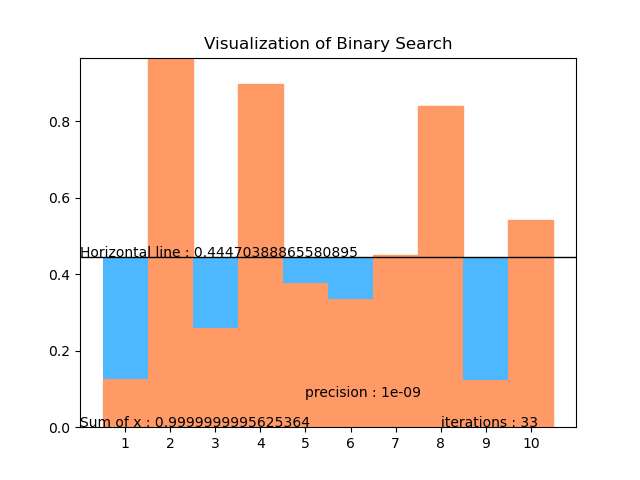
\includegraphics[width=7.8cm]{V of B.png}
            \caption{\textit{Binary Search}}
     \end{minipage}
     \begin{minipage}[H]{0.5\linewidth}
        \hspace{0.2mm}
         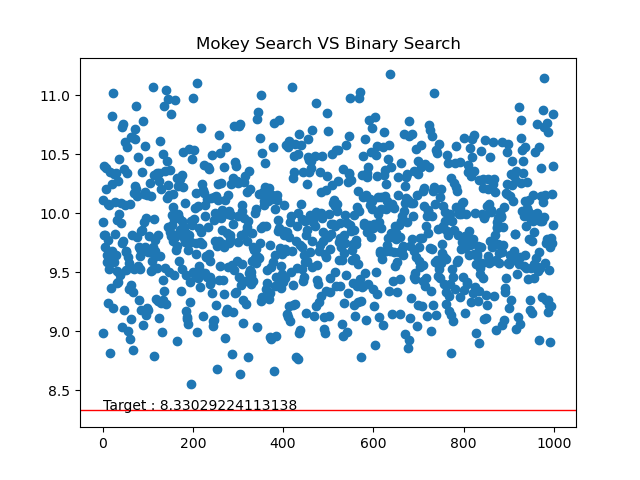
\includegraphics[width=7.8cm]{M of B.png}
         \caption{\textit{Binary Search}}
      \end{minipage}
\end{figure}

\begin{figure}[H]
    \begin{minipage}[H]{0.5\linewidth} % 图片占一行宽度0.5
            \centering
            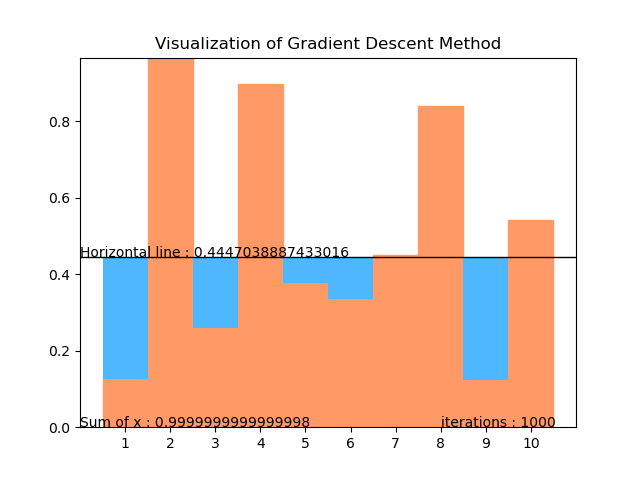
\includegraphics[width=7.8cm]{V of G.png}
            \caption{\textit{Gradient Descent Method}}
     \end{minipage}
     \begin{minipage}[H]{0.5\linewidth}
        \hspace{0.2mm}
         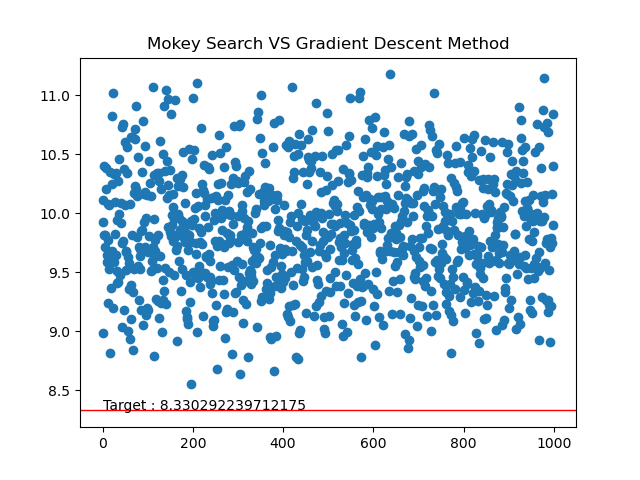
\includegraphics[width=7.8cm]{M of G.png}
         \caption{\textit{Gradient Descent Method}}
      \end{minipage}
\end{figure}

\begin{figure}[H]
    \begin{minipage}[H]{0.5\linewidth} % 图片占一行宽度0.5
            \centering
            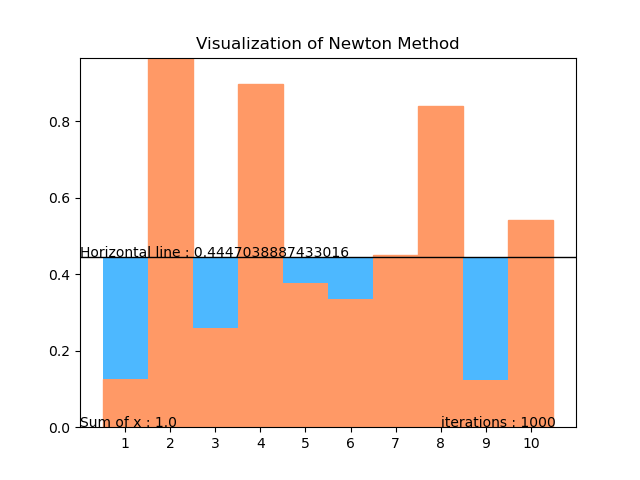
\includegraphics[width=7.8cm]{V of N.png}
            \caption{\textit{Newton Method}}
     \end{minipage}
     \begin{minipage}[H]{0.5\linewidth}
        \hspace{0.2mm}
         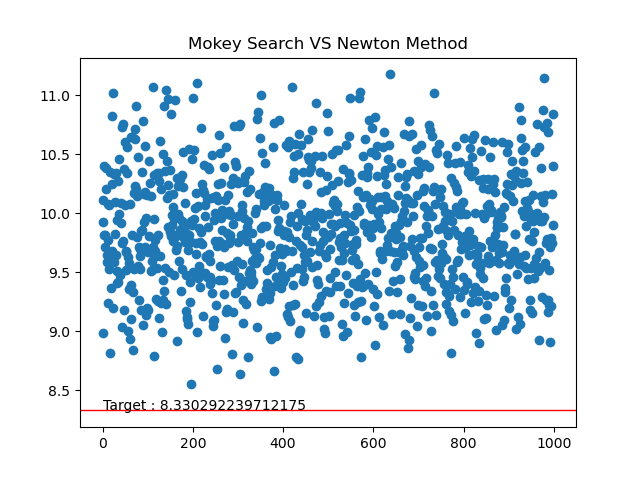
\includegraphics[width=7.8cm]{M of N.png}
         \caption{\textit{Newton Method}}
      \end{minipage}
\end{figure}
\begin{itemize}
    \item 
    {
        In \textit{Binary Search}, I set precision with $1e-9$, and we can see that it only needs $33$ iterations, which is very efficient.\\
        It turned out that sum of $x$ is $0.9999999995625364$ which is very close to $1$ and satisfies the precision and target decreases to a small number $8.33029224113138$.
    }
    \item 
    {
        In \textit{Gradient Descent Method}, I set iterations with $1000$ and used the \textit{Backtracking Line Search} with $1000$ max iteration.\\
        It turned out that the sum of $x$ is $0.9999999999999998$ which is very close to $1$ and target decreases to $8.330292239712175$ which is a little better than \textit{Binary Search}.
    }
    \item 
    {
        In \textit{Newton Method}, I set iterations with $1000$ and used the \textit{Backtracking Line Search} with $1000$ max iteration.\\
        It turned out that the sum of $x$ is $1.0$ which is very close to $1$ and target decreases to $8.330292239712175$.
    }
\end{itemize}

\subsubsection{Discussion on Dimension $n$}
\begin{table}[H]
    \begin{center}
      \caption{Binary Search}
      \begin{tabular}{c|c|c|c} % <-- Alignments: 1st column left, 2nd middle and 3rd right, with vertical lines in between
        \textbf{dimension $n$} & \textbf{iterations} & \textbf{sum of $x$} & \textbf{target}\\
        \hline
        10 & 30 & 1.000000001753952 & 8.330292234022055 \\
        20 & 30 & 1.0000000009110206 & 20.652378045251726 \\
        50 & 32 & 1.0000000009443624 & 59.84541793154762 \\
        100 & 33 & 0.9999999989148151 & 127.35888574561403 \\
        200 & 33 & 0.9999999994600418 & 249.72533875828353 \\
        500 & 35 & 0.9999999997656048 & 651.7772009927137 \\
        1000 & 35 & 0.9999999996562974 & 1319.1718511257977 \\
        10000 & 42 & 0.9999999999154736 & 14023.175128139863 
      \end{tabular}
    \end{center}
\end{table}
In \textit{Binary Search}, I set precision with $1e-8$.

\begin{table}[H]
    \begin{center}
      \caption{Gradient Descent Method}
      \begin{tabular}{c|c|c} % <-- Alignments: 1st column left, 2nd middle and 3rd right, with vertical lines in between
        \textbf{dimension $n$} & \textbf{sum of $x$} & \textbf{target}\\
        \hline
        10 & 0.9999999999999998 & 8.330292239712175 \\
        20 & \textbf{0.9999999999999997} & 20.652378049182065 \\
        50 & \textbf{1.0} & 59.84541793759993 \\
        100 & \textbf{1.0} & 127.35888573539113 \\
        200 & \textbf{1.0} & 249.7253387515363 \\
        500 & \textbf{0.9999999999999998} & 651.7772009878523 \\
        1000 & \textbf{1.0} & 1319.171851116217 \\
        10000 & \textbf{0.9999999999999996} & 14023.175128131234 
      \end{tabular}
    \end{center}
\end{table}
In \textit{Gradient Descent Method}, I set max iterations with $1000$.

\begin{table}[H]
    \begin{center}
      \caption{Newton Method}
      \begin{tabular}{c|c|c} % <-- Alignments: 1st column left, 2nd middle and 3rd right, with vertical lines in between
        \textbf{dimension $n$} & \textbf{sum of $x$} & \textbf{target}\\
        \hline
        10 & \textbf{1.0} & 8.330292239712175 \\
        20 & 0.9999999999999991 & 20.65237804918207 \\
        50 & 0.9999999999999986 & 59.84541793759995 \\
        100 & 0.9999999999999957 & 127.35888573539121 \\
        200 & 0.9999941080478836 & 249.72553013269402 \\
        500 & 0.9297244906311094 & 658.2840629609998 \\
        1000 & 0.5782796887567309 & 1353.8930686187957 \\
        10000 & 0.615221710576339 & 14221.123470723647
      \end{tabular}
    \end{center}
\end{table}
In \textit{Newton Method}, I set max iterations with $1000$ as the same.
\begin{itemize}
    \item From table 1, we find out that in \textit{Binary Search} with parameter \textit{precision} fixed, as the dimension grows, the iterations grows slowly, but is always efficient.
    \item From table 2 and the results in monkey search, we were surprised to find that the performence of \textit{Gradient Descent Method} is almost unaffected by the dimension.
    \item 
    {
        From table 3, we can see that as the dimension grows, the sum of $x$ slowly deviates from $1$, which is a bad phenomenon.\\
        I guess this is because the number of iterations is too small, and when I set the dimension $n = 10000$ and max iterations with $100000$, the sum of $x$ turned out to become $0.9999999926158202$ with target $14023.175130704825$, which looks normal.\\ 
        The reason I guess is that \textbf{As the \textit{Newton Method} proceeds, the step size should decrease, otherwise we may choosed a big step and made the sum of $x$ decreases a lot}.\\
        In order to confirm my guess, I set the max iteration with $1000$, dimension $n = 10000$ and discuss on the initial step in \textit{Backtracking Line Search}.
        \begin{table}[H]
            \begin{center}
              \caption{Discussion on Initial Step Size in \textit{Backtracking Line Search}}
              \begin{tabular}{c|c|c} % <-- Alignments: 1st column left, 2nd middle and 3rd right, with vertical lines in between
                \textbf{initial step size} & \textbf{sum of $x$} & \textbf{target}\\
                \hline
                1.0 & 0.615221710576339 & 14221.123470723647 \\
                0.8 & \textbf{0.9842580219785946} & \textbf{14219.855889521325} \\
                0.5 & 0.615221710576339 & 14221.123470723647 \\
                0.1 & \textbf{0.9842580219785946} & \textbf{14219.855889521325} \\
                0.01 & 0.7874384545583886 & 14220.531921277568                 
              \end{tabular}
            \end{center}
        \end{table}
        From the table, interestingly, different initial step size may obtian the same result, and it not that the smaller initial step sieze the better performence. 
    }
\end{itemize}


\subsection{Vertical Comparision}
In this comparision, I fixed $n = 10$, then set a series of parameters of of each method and compare their impact. In this part, the random seed is still $123456$.
\subsubsection{Binary Search}
\begin{table}[H]
    \begin{center}
      \caption{Binary Search}
      \begin{tabular}{c|c|c|c} % <-- Alignments: 1st column left, 2nd middle and 3rd right, with vertical lines in between
        \textbf{precision} & \textbf{iterations} & \textbf{sum of $x$} & \textbf{target}\\
        \hline
        1e-1 & 7 & 0.9854959700589823 & 8.37749991528356 \\
        1e-2 & 10 & 0.9964362155179058 & 8.341863037752896 \\
        1e-3 & 13 & 0.9996475623041371 & 8.331435698156694 \\
        1e-4 & 17 & 1.0000209098077328 & \textbf{8.330224405058946} \\
        1e-5 & 20 & 1.000002957539133 & 8.330282644958652 \\
        1e-6 & 23 & 0.9999998159219318 & 8.330292836892756 \\
        1e-7 & 27 & 1.0000000122727468 & 8.330292199897297 \\
        1e-8 & 30 & 1.000000001753952 & 8.330292234022055 \\
        1e-9 & 33 & 0.9999999995625364 & 8.33029224113138 \\
        1e-10 & \textbf{37} & \textbf{0.9999999999734269} & 8.33029223979838 \
      \end{tabular}
    \end{center}
\end{table}
\begin{itemize}
    \item From the table above, it is easy to find that the number of iterations and the precision of difference between sum of $x$ and $1$ is directly related to the parameter \emph{precision}.
    \item And performence of \emph{target} may be rarely associated with parameter \emph{precision}.
\end{itemize}

\subsubsection{Gradient Descent Method}
In analysis below, I made two comparisions: the max iterations and using backtracking line search or not. I do not consider the iterations in backtracking line search, because it will always ends in a small number of iterations.
\begin{table}[H]
    \begin{center}
      \caption{Gradient Descent Method using Backtracking Line Search}
      \begin{tabular}{c|c|c} % <-- Alignments: 1st column left, 2nd middle and 3rd right, with vertical lines in between
        \textbf{iterations} & \textbf{sum of $x$} & \textbf{target}\\
        \hline
        1 & 0.5996978112837809 & 10.046418174429736 \\
        5 & 0.9866644124857917 & 8.430947441250991 \\
        10 & 0.9997781218498675 & 8.334272506259687 \\
        20 & 0.9999845516531557 & 8.33034869077645 \\
        50 & 0.9999999999994104 & 8.330292239714463 \\
        100 & \textbf{0.9999999999999998} & \textbf{8.330292239712175} \\
        500 & \textbf{0.9999999999999998} & \textbf{8.330292239712175} \\
        1000 & \textbf{0.9999999999999998} & \textbf{8.330292239712175} \\
        10000 & \textbf{0.9999999999999998} & \textbf{8.330292239712175} 
      \end{tabular}
    \end{center}
\end{table}
From the table above, it is easy to find out that the convergence speed is impressive, and saturation is reached after almost $100$ iterations.

\begin{table}[H]
    \begin{center}
      \caption{Gradient Descent Method with Fixed Stepsize}
      \begin{tabular}{c|c|c} % <-- Alignments: 1st column left, 2nd middle and 3rd right, with vertical lines in between
        \textbf{stepsize} & \textbf{sum of $x$} & \textbf{target}\\
        \hline
        1e-1 & 136.68263799843982 & -38.237979542758495 \\
        1e-2 & 39.8889399957294 & -21.63855225777158 \\
        1e-3 & 9.401411836686217 & -5.1838843477010155 \\
        1e-4 & \textbf{1.324753676483748} & \textbf{7.338759167059794} \\
        1e-5 & 0.2820381305500916 & 11.226990829633314 \\
        1e-6 & 0.205025479153595 & 11.67804173573701 \\
        1e-7 & 0.19702955018123156 & 11.729147183266553 
      \end{tabular}
    \end{center}
\end{table}
In the experiments above, I set max iterations with $1000$, and the performence looks bad. 

\subsubsection{Newton Method}
In analysis below, I made comparisions among different max iterations and do not consider the iterations in backtracking line search.
\begin{table}[H]
    \begin{center}
      \caption{Newton Method using Backtracking Line Search}
      \begin{tabular}{c|c|c} % <-- Alignments: 1st column left, 2nd middle and 3rd right, with vertical lines in between
        \textbf{iterations} & \textbf{sum of $x$} & \textbf{target}\\
        \hline
        1 & 0.8359152954500617 & 10.035688630176235 \\
        5 & 0.8423697957445522 & 9.286513603368162 \\
        10 & 0.9562616963351661 & 8.55558788241405 \\
        20 & 0.9984104159780414 & 8.337795046131635 \\
        50 & 0.9999999098836335 & 8.330292674682592 \\
        100 & 0.9999999999999952 & 8.330292239712206 \\
        500 & \textbf{1.0} & \textbf{8.330292239712175} \\
        1000 & \textbf{1.0} & \textbf{8.330292239712175} \\
        10000 & \textbf{1.0} & \textbf{8.330292239712175} 
      \end{tabular}
    \end{center}
\end{table}
From the table above, it is easy to see that the convergence speed is impressive, and saturation is reached after almost $100$ iterations. 

\subsection{Visualization of Iteration Process}
In this part, I select two random seed $123456$ and $12345$, and compare the process of these methods.
\begin{figure}[H]
    \begin{minipage}[H]{0.5\linewidth} % 图片占一行宽度0.5
            \centering
            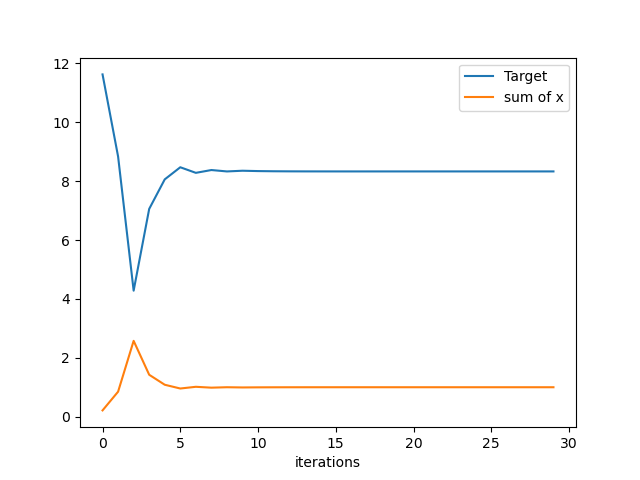
\includegraphics[width=7.8cm]{T of B1.png}
            \caption{\textit{Binary Search 1}}
     \end{minipage}
     \begin{minipage}[H]{0.5\linewidth}
        \hspace{0.2mm}
         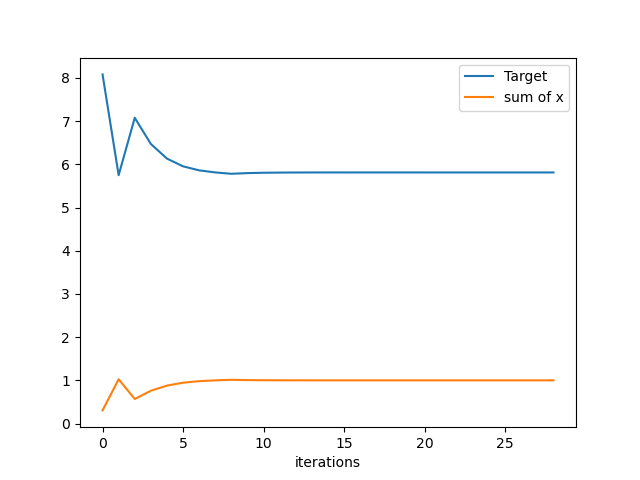
\includegraphics[width=7.8cm]{T of B2.png}
         \caption{\textit{Binary Search 2}}
      \end{minipage}
\end{figure}
\begin{figure}[H]
    \begin{minipage}[H]{0.5\linewidth} % 图片占一行宽度0.5
            \centering
            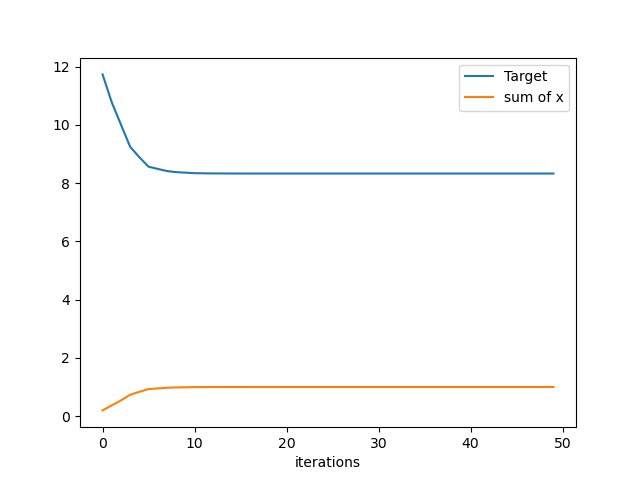
\includegraphics[width=7.8cm]{T of G1.png}
            \caption{\textit{Gradient Descent Method 1}}
     \end{minipage}
     \begin{minipage}[H]{0.5\linewidth}
        \hspace{0.2mm}
         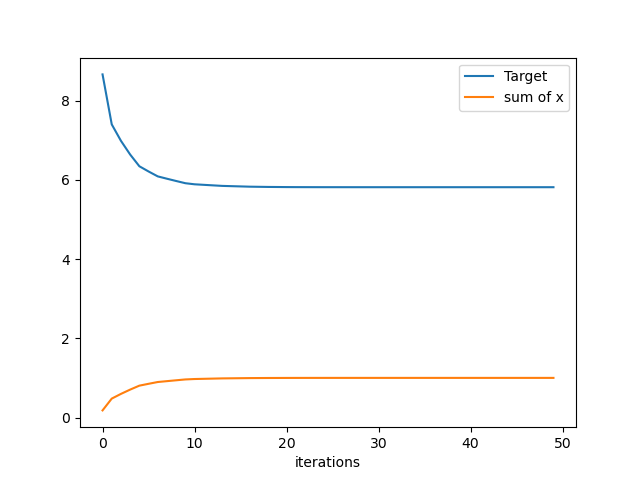
\includegraphics[width=7.8cm]{T of G2.png}
         \caption{\textit{Gradient Descent Method 2}}
      \end{minipage}
\end{figure}
\begin{figure}[H]
    \begin{minipage}[H]{0.5\linewidth} % 图片占一行宽度0.5
            \centering
            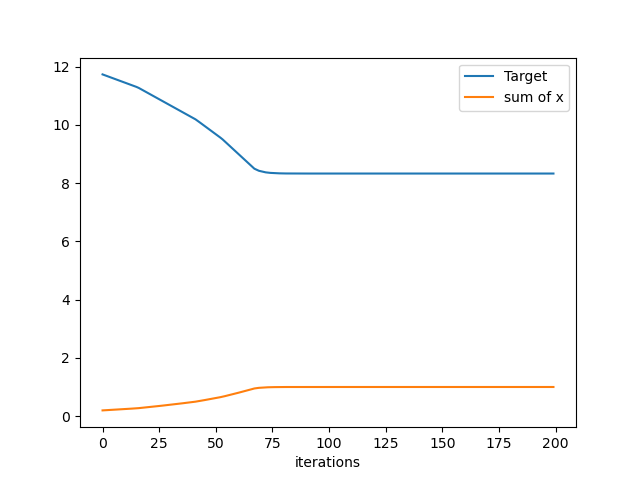
\includegraphics[width=7.8cm]{T of N1.png}
            \caption{\textit{Newton Method 1}}
     \end{minipage}
     \begin{minipage}[H]{0.5\linewidth}
        \hspace{0.2mm}
         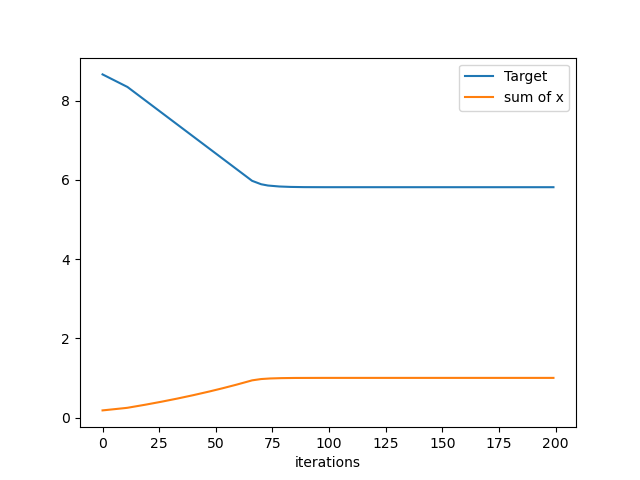
\includegraphics[width=7.8cm]{T of N2.png}
         \caption{\textit{Newton Method 2}}
      \end{minipage}
\end{figure}
In the graph above, $1$ means we used random seed $123456$ and $2$ is $12345$.\\
\begin{itemize}
    \item It is apparent that the \textit{Binary Search} moves fast, but is not stable in the beginning.
    \item 
    {
        And the \textit{Gradient Descent Method} converge faster than \textit{Newton Method}, 
        the reason I guess is: \textbf{Since \textit{Newton Method} uses the \textit{Taylor} second-order term,which is quadratic, 
        the rate of descent is significant while $x$ is far from $x_{opt}$, and it slows down while $x$ is getting close to $x_{opt}$}.
        And in this problem, $x$ is always \textit{near} $x_{opt}$.
    }
\end{itemize}





\section{Conclusion}
In this project, we made a deep analysis of the original problem first and use strategies learned from class converting it into a more straightward problem -- the water filling problem. 
Next, we used three different methods to solve it, and made some clear and intuitive comparisions and analysis.

From this project, I gained a deeper understanding of handling optimization problems, it helped me learn to see optimization problems from a different perspective, I hold a firm belief that this will be of great benefit to my future study and life.

\end{document}